\documentclass[11pt]{article}
\usepackage{graphicx}
\usepackage{hyperref}
\usepackage{natbib}
\usepackage{amsmath}
\usepackage{enumitem}
\usepackage{mathtools}

\setlength{\textwidth}{6.5in}
\setlength{\headheight}{0in}
\setlength{\textheight}{8.0in}
\setlength{\hoffset}{0in}
\setlength{\voffset}{0in}
\setlength{\oddsidemargin}{0in}
\setlength{\evensidemargin}{0in}

\title{PS10}
  
\author{Shihong Pan\\ \url{https://github.com/PSH-hub24/phys-ga2000}}


\begin{document}

\maketitle

\section*{Q1}
The instructions are pretty detailed in this assignment. I used banded.py to solve the linear system. However I couldn't get VPython working, so I instead plotted $\psi$ at at 0 steps, 1000 steps, and 5000 steps. I also scaled the y-axis by 1e-9 as recommended by the instruction. Fig \ref{fig:Q1} shows a drift in the wavefunction as time increases, i.e., the region where the electron resides with high probability drifts in time. 

\section*{Q2}
I used dcst.py as instructed. Fig \ref{fig:Q2b} plots $\psi$ at  $t=10^{-16}$s, calculated by using the given formula and idst respectively. They match pretty well. Fig \ref{fig:Q2cd} plots the evolution of $\psi$, again a few snapshot since I couldn't get VPython working. The plot also shows a drift in the region where the electron moves with high probability, which matches the result in Q1.

\begin{figure}[b!]
\centering
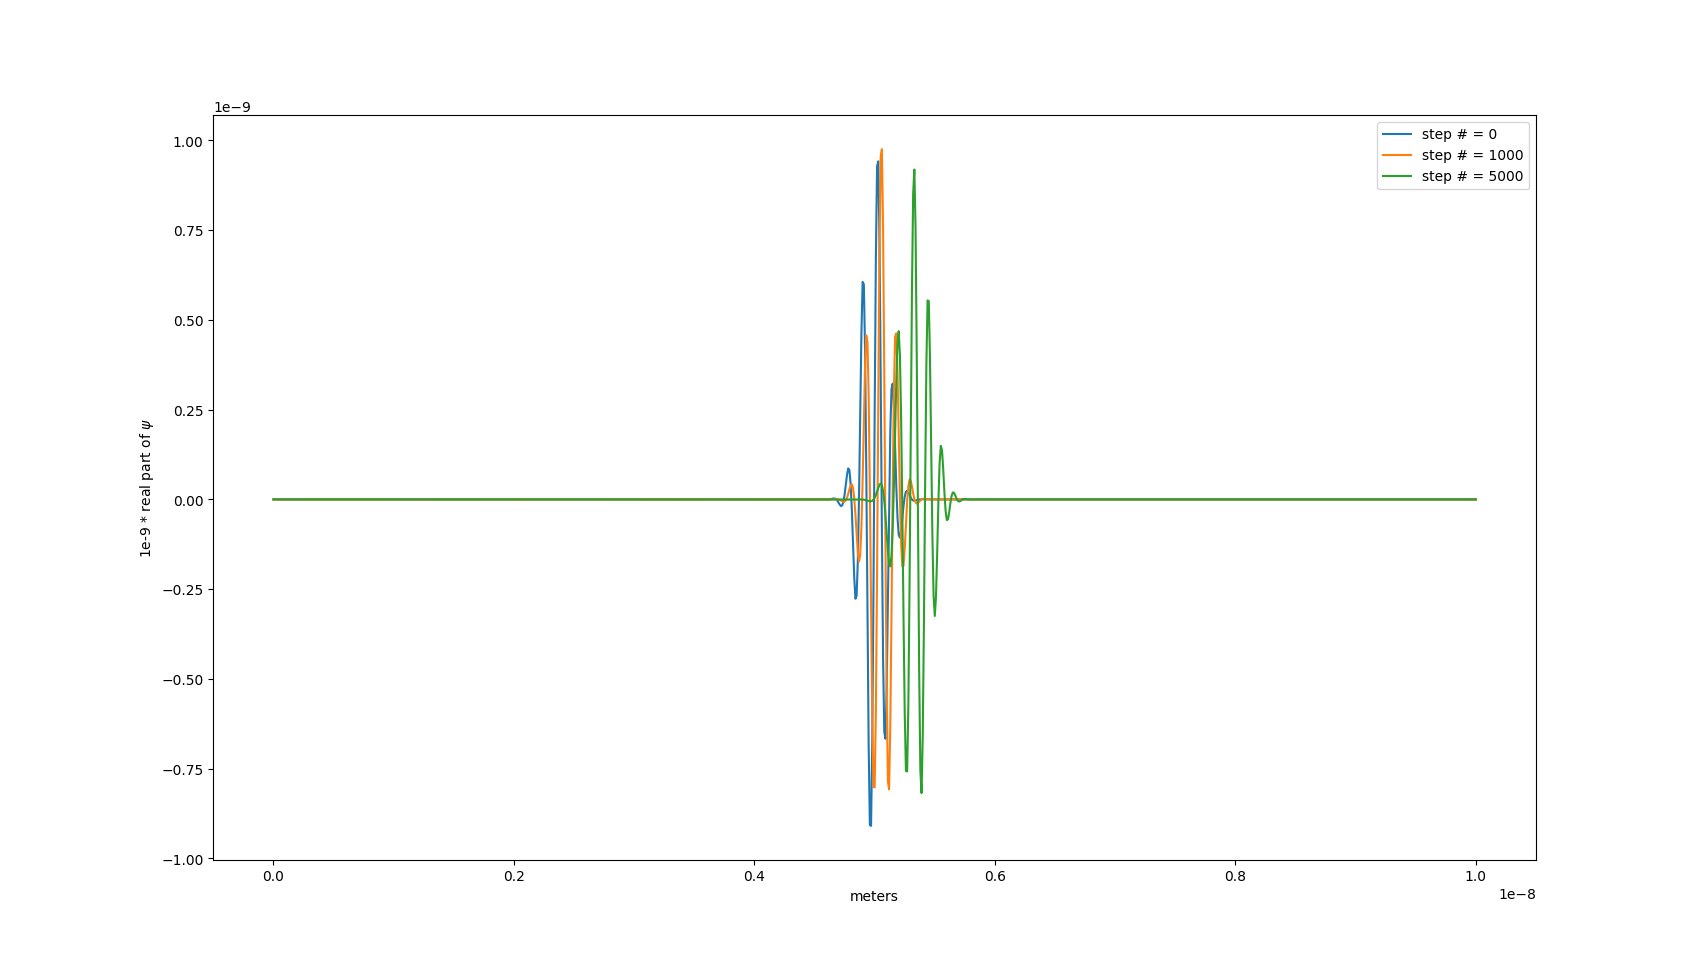
\includegraphics[width=1\textwidth]{Computational Physics/ps10Figures/q1.png}
\caption{The real part of $\psi$ at 0 steps, 1000 steps, and 5000 steps.}
  \label{fig:Q1}
\end{figure}

\begin{figure}[b!]
\centering
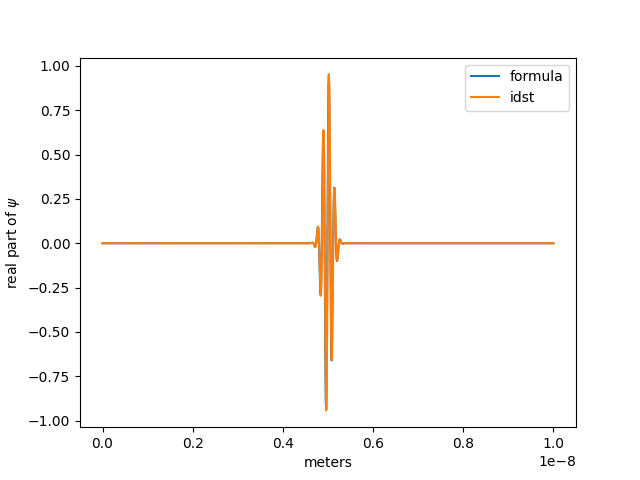
\includegraphics[width=1\textwidth]{Computational Physics/ps10Figures/q2b.png}
\caption{$\psi$ at $t=10^{-16}$s, calculated by the given formula and idst respectively.}
  \label{fig:Q2b}
\end{figure}

\begin{figure}[b!]
\centering
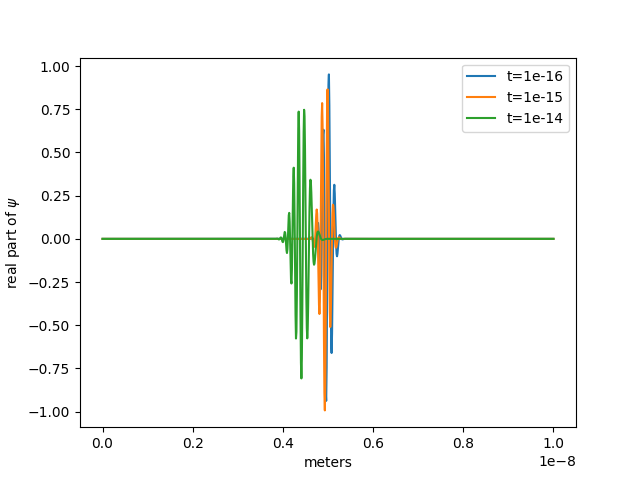
\includegraphics[width=1\textwidth]{Computational Physics/ps10Figures/q2d.png}
\caption{Time evolution of $\psi$}
  \label{fig:Q2cd}
\end{figure}





\bibliographystyle{apj}
\bibliography{example}

\end{document}

 
 
